\documentclass[lettersize,journal]{IEEEtran}
\usepackage{amsmath,amsfonts}
\usepackage{algorithmic}
\usepackage{array}
\usepackage[caption=false,font=normalsize,labelfont=sf,textfont=sf]{subfig}
\usepackage{textcomp}
\usepackage{stfloats}
\usepackage{url}
\usepackage{verbatim}
\usepackage{graphicx}
\usepackage{titlesec}
\hyphenation{op-tical net-works semi-conduc-tor IEEE-Xplore}
\def\BibTeX{{\rm B\kern-.05em{\sc i\kern-.025em b}\kern-.08em
    T\kern-.1667em\lower.7ex\hbox{E}\kern-.125emX}}
\usepackage{balance}
%\usepackage{natbib}
\usepackage{cite}
\usepackage{tabularx}
\hyphenpenalty=25
\tolerance=10000
\allowdisplaybreaks[4]
\usepackage{tcolorbox}
\usepackage{enumitem}
\newcommand{\ciao}[1]{{\setlength\fboxrule{0pt}\fbox{\tcbox[colframe=black,colback=white,shrink tight,boxrule=0.5pt,extrude by=1mm]{\small #1}}}}
% \usepackage{fontspec}
% \usepackage{libertine}

\usepackage{etoolbox}
\makeatletter
\patchcmd{\@makechapterhead}{\cleardoublepage}{}{}{}
\makeatother

\setlength{\abovedisplayskip}{1ex}
\setlength{\belowdisplayskip}{1ex}

\usepackage[colorlinks=true,linkcolor=black,citecolor=blue,urlcolor=blue,]{hyperref}


\begin{document}

\title{\fontsize{20pt}{24pt}\selectfont Unlocking Flexibility Potential through DVFS-controlled Data Center Clusters in Unit Commitment}
\author{Yufei Teng, Member, \textit{IEEE}, Yiping Yuan, Member, \textit{IEEE}, Liqian Zhu, Student Member, \textit{IEEE}, Yihang Cao, Student Member, \textit{IEEE}, Zhenyuan Zhang, Senior Member,~\textit{IEEE}}

\IEEEaftertitletext{\vspace{-1.0\baselineskip}}

\markboth{Journal of \LaTeX\ Class Files,~Vol.~18, No.~9, September~2020}%
{How to Use the IEEEtran \LaTeX \ Templates}

\maketitle

\begin{abstract}
  Data center clusters (DCCs) have become recognized as significant energy consumers in electrical power system operations. Workload balancing for DCCs, implemented by dynamic voltage and frequency scaling (DVFS) control schemes, allows for providing flexibility potential capability and contributes to maintaining the security of scheduling results through Unit Commitment (UC).
  To achieve this, the flexibility potential of DCCs under different workload conditions is analyzed. Building on this analysis, a new set of physical constraints representing workload balancing across multiple DVFS-controlled DCCs is proposed, and related linearized constraints is extended through McCormick Envelopes method. Furthermore, these intractable constraints are incorporated into UC, and an enhanced UC (EUC) model, which considers the flexibility potential offered by DVFS-controlled DCCs, is developed. Several experiments are conducted on the IEEE 6 bus and 118 bus test systems to assess the validity and scalability of the proposed models.

\end{abstract}

\begin{IEEEkeywords}
  Data center clusters, Flexibility Capability, Enhanced Unit Commitment, McCormick Envelopes
\end{IEEEkeywords}

\vspace{-0.5cm}

\section{Introduction}
\IEEEPARstart{A}{s} the increase in various artificial intelligence technologies and demand energy consumptions, the operation of electrical power systems are becoming diverse and uncontrollable, and they are facing challenges in provide sufficient flexible adjustment resources against emergence events~\cite{6041050,7039172}. In such circumstances, additional flexible mechanisms such as demand response, virtual Power plant, and energy storage systems, etc., needs to be prioritized. Nevertheless, as a significant energy consumer, DCCs have not been fully utilized in the flexibility potential of power system operations. To this end, it it essential to investigate the flexible adjustment characteristic of DCCs, and to explore the potential of DCCs in providing flexible adjustment resources for the economic and reliable operation of electrical power systems.

Recent literature reported several studies on the DCCs flexibility modeling and its application in electrical power systems operation. Specially, 
Ref.~\cite{10874152} carried out a Quality-of-service-based cost function to describe the workload shifting and server utilization of DCCs, and extended a distributed dispatch framework with considering DCCs flexibility.
Ref.~\cite{6041050} designed a mix-integer programming model to achieve the the optimal demand management of DCCs.
Ref.~\cite{7039172} analyzed the progressive load characteristics in DCCs, and proposed two optimization models to estimate the optimal capability planning of storage systems in DCCs and design parameters optimizations.
Ref.~\cite{10806734} explored the statistical feasibility of DDCs and hydrogen resources in a microgrid context, and carried out a data-driven statistical-feasibility-based robust rolling optimization framework to analysis the optimal operation of DDCs and hydrogen storage systems under complex uncertain factors.
Ref.~\cite{doi:10.1049/icp.2025.0664} further analyzed the potential capability of DDCs for regulating computational workloads while reducing carbon emissions, and then constructed a emission-aware coordinated dispatch method of multi-regional microgrids with DDCs.
The aforementioned studies primarily emphasize the flexibility ability of DCCs within electrical power system operations. However, they often overlook the intricate physical characteristics of DCCs, particularly in relation to workload shifting dynamics and the implementation of advanced high-evolution control strategies.

The workloads in DCCs can be broadly classified into three categories, \cite{6041050}, $i$) $compute$-$intensive$ $workloads$, which include high-performance computing (HPC), machine learning model training, and commercial application services. $ii$) $storage$-$intensive$ $workloads$, which are employed for tasks such as regular file backups, archival systems, and relational database applications. $iii$) $network$-$intensive$ $workloads$, encompassing activities like website hosting, content delivery networks, and network traffic management. Notably, compute-intensive and storage-intensive workloads dominate in DCCs, collectively accounting for approximately $70$\% of the total workload. This dominance is driven by the growing demand for HPC and data-driven techniques. In contrast, network-intensive workloads are typically less predictable and highly time-sensitive, requiring immediate processing to ensure seamless operation. Since the former two workloads are more predictable and flexible, the peak workload requirements of the former two workloads can be effectively shifted or adjusted through DVFS, \cite{lin2023workload,7039172,6041050}, to achieve load balancing and energy management.

Driven by such motivation, this paper constructs a set of DVFS-controlled DCCs physical constraints for representing their flexible characteristics under various workload configurations, and further extends an EUC model to reflect proactive flexibility supplement of DCCs. The main contributions of this paper are summarized as follows,
$i$) A DVFS-controlled physical constraints is developed to characterize the flexibility attributes of DCCs workloads. Furthermore, the proposed constraints are linearized using McCormick Envelopes to enhance computational tractability in UC studies.
$ii$) A EUC model is formulated to capture the dynamic flexible response of DCCs. The model incorporates a new coordination mechanism to address multi-timescale interactions between workload shifting in DCCs and grid-side demand fluctuations.

The remainder of this abstract is organized as follows. Section II outlines the scheduling framework for power systems, incorporating the consumption characteristics of DCCs workloads. Section III proposed DVFS-controlled physical constraints, and lists a detailed formulation of the proposed EUC model.
% Section IV presents numerical experiments to demonstrate the effectiveness and practicality of the proposed model.

\vspace{-0.25cm}
\section{The proposed Scheduling Framework}

This section presents a coordinated scheduling framework designed to integrate the flexible response capabilities of DCCs. Recognizing the difference in scheduling timescales (hourly for grid-side operations versus seconds for DCCs workload management), the framework is structured into two interconnected parts. PART-1 encompasses the grid-side scheduling model, while PART-2 represents the DCCs workload management model.

%Part-1 optimizes the power system's generation schedule, and Part-2 optimizes workload shifting within DCCs.

\begin{figure}[!h]
    \centering
    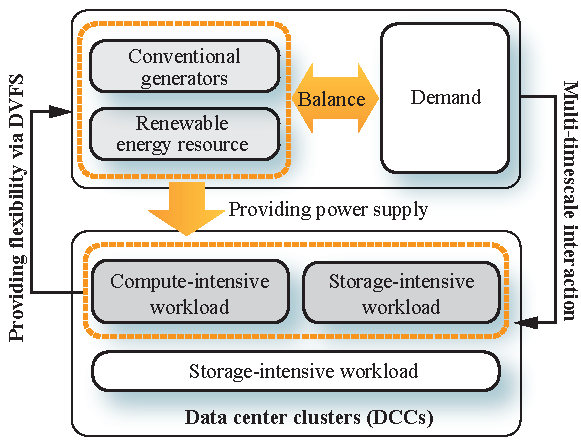
\includegraphics[width=0.425\textwidth]{./fig/framework.pdf}\vspace{-0.35cm}
    \caption{The proposed scheduling framework in this work}\vspace{-0.35cm}
    \label{fig:sfr}
  \end{figure}

\vspace{-0.25cm}
\section{reformulated constraints for DVFS-controlled DCCs}

The power consumption of DCCs is primarily influenced by two components: static energy and dynamic energy. The static energy, often referred to as idle power, arises mainly from the leakage current in the CPU core circuits. In contrast, the dynamic energy is predominantly determined by the workload ratio $\lambda_{dcc}$ and the individual service level $\mu_{dcc}$. The total power consumption of DCCs can be expressed as follows, \cite{lin2023workload},

\vspace{-0.25cm}
\begin{subequations}
  \begin{align}
    p_{dcc,i} &= p_{dcc,i}^{idle} + p_{dcc,i}^{dyn},\forall i\in\mathcal{I}\\
    p_{dcc,i}^{idle} &= v_{dcc,i} i_{leak},\forall i\in\mathcal{I}\\
    p_{dcc,i}^{dyn} &= {\left( C_{dcc,i} f_{dcc,i} v_{dcc,i}^{2} \right )}{\lambda_{dcc,i}}{\mu_{dcc,i}^{-1}}, \forall i\in \mathcal{I}
  \end{align}
\end{subequations}

\noindent
where $i$ and $\mathcal{I}$ represent the index and set of DCCs. $p_{dcc,i}$ denotes the total power consumption of individual DCC $i$. $p_{dcc,i}^{idle}$ and $p_{dcc,i}^{dyn}$ represent the static (idle) and dynamic power consumption of DCC $i$, respectively. $C_{dcc,i}$ defines the constant representing the effective capacitance of DCC $i$. $f_{dcc,i}$ and $v_{dcc,i}$ denote the operational frequency and voltage of DCC $i$, respectively.

Based on the above physical working principles, the set of physical security constraints representing DCCs workflows can be extended,

\vspace{-0.25cm}
\begin{subequations}
  \begin{align}
    p_{dcc,i} & \!\geq\! p_{dcc,i}^{idle} \!+\! p_{dcc,i}^{dyn},\forall i\in\mathcal{I}\\
    p_{dcc,i}^{idle} &\!\geq\! \lfloor {v}_{dcc,i}\rfloor i_{leak},p_{dcc,i}^{idle} \!\leq\! \lceil {v}_{dcc,i}\rceil i_{leak},\forall i\in\mathcal{I}\\
    p_{dcc,i}^{dyn}& \!\geq\! \lfloor \phi_{dcc,i}^{dvfs} \rfloor {\lambda_{dcc,i}}{\mu_{dcc,i}^{-1}}, p_{dcc,i}^{dyn} \!\leq\! \lceil \phi_{dcc,i}^{dvfs} \rceil {\lambda_{dcc,i}}{\mu_{dcc,i}^{-1}},\notag \\
    \phi_{dcc,i}^{dvfs} &= ( C_{dcc,i} f_{dcc,i} v_{dcc,i}^{2} ), \forall i\in \mathcal{I}
  \end{align}
\end{subequations}

\noindent
where $\lceil {\circ} \rceil$ and $\lfloor {\circ} \rfloor$ represent pre-determined upper and lower bounds for the decision variable $\circ$. The term $\phi_{dcc,i}^{dvfs}$ represents the power regulation process for the DCC $i$ through DVFS technique, while $\lambda_{dcc,i}$ describes the workload balancing process for the DCC $i$. The feasibility of workload balancing for compute-intensive and storage-intensive workloads hinges on users' latency tolerance for batch workloads and the capacity to shift workloads among DCCs. When users accept tolerate higher latency, the execution of workloads can be dynamically adjusted across multi DCCs. By optimizing these workload execution patterns, the overall energy consumption of DCCs can be optimized through DVFS and sequentially reduced, thereby enhancing their demand response capabilities for power system operations.

To reflect it, additional concise constraints concerning workload balancing processes among multi DCCs are constructed,

\vspace{-0.25cm}
\begin{subequations}
  \begin{align}
    \varDelta p_{dcc,i}^{bal} = \phi_{dcc,i}^{dvfs} {\left ( \lambda_{dcc,i}^{ini} + \varDelta \lambda_{dcc,i}\right )}{\mu_{dcc,i}^{-1}}, \forall i\in \mathcal{I}\\
    p_{dcc,i} \geq p_{dcc,i}^{idle} \!+\! p_{dcc,i}^{dyn} + \varDelta p_{dcc,i}^{bal},\forall i\in\mathcal{I}\\
    \sum\nolimits_{t\in\mathcal{T}} \sum\nolimits_{i\in\mathcal{I}} \varDelta \lambda_{dcc,i} = 0, \forall i\in\mathcal{I}, \forall t\in\mathcal{T}\\
    \lfloor f_{dcc,i} \rfloor \leq f_{dcc,i} \leq \lceil f_{dcc,i} \rceil, \forall i\in \mathcal{I}\\
    \lfloor v_{dcc,i} \rfloor \leq v_{dcc,i} \leq \lceil v_{dcc,i} \rceil, \forall i\in \mathcal{I}
  \end{align}
\end{subequations}

\noindent
where $\varDelta p_{dcc,i}^{bal}$ represents the change in the power consumption for DCC $i$ due to workload balancing, $\lambda_{dcc,i}^{ini}$ represents the initial workload, and $\varDelta \lambda_{dcc,i}$ represents the adjusted workload. By incorporating the workload balancing dynamics defined in (3a)-(3c) into (2b) and (2c), the form of DVFS-controlled DCCs constraints can be established.
Despite these constraints, these constraints remains elusive due to the presence of product terms involving continuous variables $\phi_{dcc,i}^{dvfs}$ and $\varDelta \lambda_{dcc,i}$ in (3a), therefore, the McCormick Envelope method is further extended and then integrated into UC studies. On this basis, an union form of EUC considering DVFS-controlled DDCs is listed below,

\vspace{-0.25cm}
\begin{subequations}
  \begin{align}
    \text{\textbf{objective function}}: & \text{minimize operation cost}\\
      \text{\textbf{security constraints}}: & \left \{\!\!\!\! \begin{array}{l}\text{system-wide power balance,}\\ 
        \text{units output bindings,}\\
        \text{and network power flow, etc.}\end{array}\right.\\
        \text{\textbf{DCCs constraints}}:& (2b),(2c), and\, (3a)-(3e)
  \end{align}
\end{subequations}


\bibliographystyle{IEEEtran}
\bibliography{IEEEabrv,reference}

\end{document}


